\documentclass[tikz, border=2pt]{standalone}
\usepackage{tikz}
\usetikzlibrary{arrows.meta,positioning,fit,backgrounds,calc,shapes.geometric}
% Shared TikZ style, color-matched to paper/figures/*.pdf (matplotlib):
% ink = near-black strokes/fill, accent = deep red for the one thing per
% diagram that should draw the eye, grid = light gray for structure that
% should recede.
\definecolor{ink}{HTML}{1A1A1A}
\definecolor{accent}{HTML}{A6192E}
\definecolor{gridgray}{HTML}{D9D9D9}
\definecolor{panelbg}{HTML}{F2F2F2}

\tikzset{
  every node/.style={font=\sffamily},
  box/.style={draw=ink, thick, rounded corners=1.5pt, minimum height=0.75cm,
              font=\sffamily\small, align=center, fill=white, text=ink},
  stubbox/.style={box, draw=ink, dashed, fill=panelbg},
  hibox/.style={box, fill=ink, text=white},
  panel/.style={draw=none, fill=panelbg, rounded corners=2pt},
  arr/.style={-{Latex[length=2.2mm, width=1.6mm]}, thick, draw=ink},
  darr/.style={arr, dashed},
  accarr/.style={-{Latex[length=2.2mm, width=1.6mm]}, thick, draw=accent},
  lbl/.style={font=\sffamily\scriptsize, text=ink},
  ital/.style={font=\sffamily\itshape\scriptsize, text=ink!70},
  note/.style={font=\sffamily\scriptsize, align=left, text=ink},
  state/.style={draw=ink, thick, rounded corners=3pt, minimum width=2.6cm,
                minimum height=0.9cm, font=\sffamily\small, align=center, fill=white},
  finalstate/.style={state, fill=ink, text=white},
  abortstate/.style={state, draw=accent, thick, text=accent},
}

\tikzset{
  dec/.style={draw=ink, thick, diamond, aspect=2.4, align=center, font=\sffamily\scriptsize,
              fill=white, inner sep=2pt, text width=2.3cm},
}
\begin{document}
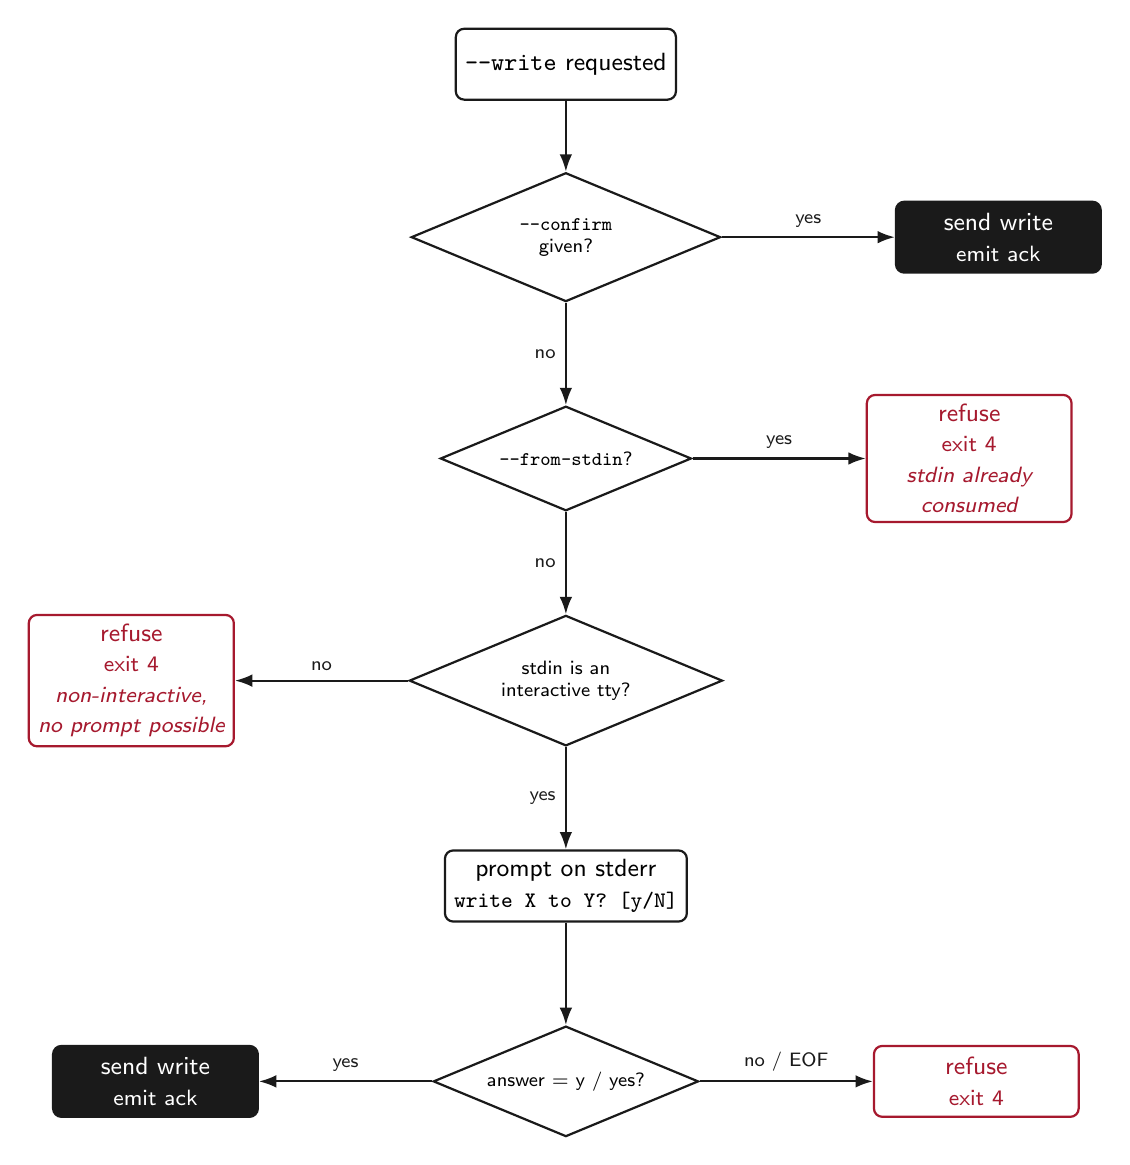
\begin{tikzpicture}[node distance=9mm and 11mm]

\node[state] (start) {\texttt{--write} requested};
\node[dec, below=of start] (confirm) {\texttt{-{}-confirm}\\given?};
\node[finalstate, right=22mm of confirm] (exec) {send write \\ \footnotesize emit ack};

\node[dec, below=13mm of confirm] (stdin) {\texttt{-{}-from-stdin}?};
\node[abortstate, right=22mm of stdin] (abort1) {refuse \\ \footnotesize exit 4 \\ \footnotesize\itshape stdin already \\ \footnotesize\itshape consumed};

\node[dec, below=13mm of stdin] (tty) {stdin is an \\ interactive tty?};
\node[abortstate, left=22mm of tty] (abort2) {refuse \\ \footnotesize exit 4 \\ \footnotesize\itshape non-interactive, \\ \footnotesize\itshape no prompt possible};

\node[state, below=13mm of tty] (prompt) {prompt on stderr \\ \footnotesize\ttfamily write X to Y? {[}y/N{]}};
\node[dec, below=13mm of prompt] (yn) {answer \(=\) y / yes?};
\node[abortstate, right=22mm of yn] (abort3) {refuse \\ \footnotesize exit 4};
\node[finalstate, left=22mm of yn] (exec2) {send write \\ \footnotesize emit ack};

\draw[arr] (start) -- (confirm);
\draw[arr] (confirm) -- node[lbl,above]{yes} (exec);
\draw[arr] (confirm) -- node[lbl,left]{no} (stdin);
\draw[arr] (stdin) -- node[lbl,above]{yes} (abort1);
\draw[arr] (stdin) -- node[lbl,left]{no} (tty);
\draw[arr] (tty) -- node[lbl,above]{no} (abort2);
\draw[arr] (tty) -- node[lbl,left]{yes} (prompt);
\draw[arr] (prompt) -- (yn);
\draw[arr] (yn) -- node[lbl,above]{no / EOF} (abort3);
\draw[arr] (yn) -- node[lbl,above]{yes} (exec2);

\end{tikzpicture}
\end{document}
